\documentclass[11pt, a4paper]{article}

% ---- Font: Times New Roman ----
\usepackage{mathptmx}

% ---- 1.5 line spacing ----
\usepackage{setspace}
\onehalfspacing

% ---- Standard margins ----
\usepackage[margin=1in]{geometry}

% ---- Packages ----
\usepackage{graphicx}
\usepackage{tikz}
\usepackage{parskip}
\usepackage{amsmath}
\usepackage{amsfonts}
\usepackage{amssymb}
\usepackage{textcomp}
\usepackage{booktabs}
\usepackage{float}
\usepackage{hyperref}
\usepackage{caption}
\usepackage[numbers]{natbib}

\hypersetup{
    colorlinks=true,
    linkcolor=blue,
    urlcolor=red,
    citecolor=blue
}

\begin{document}

% ============================================================
% FRONT PAGE
% ============================================================
\begin{titlepage}
    \centering
    \vspace*{1.0cm}

    {\Large\textbf{INDIAN INSTITUTE OF TECHNOLOGY MADRAS}\par}
    \vspace{0.8cm}

    % IIT Madras logo: place iitm_logo.png in the same folder as this .tex file
    
\includegraphics[width=0.22\textwidth]{iitm_logo.png}\par

    \vspace{1.2cm}
    {\Large\textbf{MS5612: Real Options Valuation}\par}

    \vspace{1.0cm}
    {\rule{0.75\textwidth}{0.5pt}\par}
    \vspace{0.8cm}

    {\LARGE\textbf{Project Report}\par}
    \vspace{0.5cm}
    {\Large\textbf{Pricing Spinny's Buyback Guarantee\\as a Real Option}\par}

    \vfill

    {\large\textbf{Submitted by Group 4}\\[0.4cm]
    Ajith, Hardik, Lokesh, \& Vikranth\\[0.8cm]}

\end{titlepage}

\tableofcontents

\newpage

% ============================================================
\section{Executive Summary}
% ============================================================

This report aims to understand and price Spinny's 3-month buyback guarantee. We argue that the buyback guarantee can be modelled as a standard put option from the consumer's perspective, and we utilise three distinct approaches to price it: the fundamental (intrinsic value) approach, the Binomial option pricing model (with deterministic depreciation), and the Black-Scholes-Merton formula (both standard and depreciation-adjusted). We also reason about how Spinny's internal team would have priced it, factoring in parameters such as returning and inspection costs among many others.

The specific vehicle we analyse is the \textbf{Mahindra Bolero Neo Plus P10 (2024)}, listed on Spinny's platform at Rs.~12,83,903 with a buyback guarantee of Rs.~11,55,641. We assume volatility at 15\% p.a. and an annual depreciation of 10\%.

The report is organised as follows. Section~\ref{sec:about} introduces Spinny. Section~\ref{sec:options_basics} provides a refresher on financial and real options. Section~\ref{sec:buyback_offer} details the specific buyback guarantee. Sections~\ref{sec:pricing_fundamental} through \ref{sec:pricing_bsm_dep} present the pricing analysis under each model. We consolidate findings in Section~\ref{sec:consolidation} and conclude in Section~\ref{sec:conclusion}.


% ============================================================
\section{About Spinny}
\label{sec:about}
% ============================================================

Spinny is a private limited company that operates in the second-hand car market. It was founded in 2015 and follows a full-stack model: it purchases used cars, inspects and refurbishes them, and sells them directly to customers through its online platform and physical car hubs \cite{forbesindia2023}. Spinny focuses on making used-car sales more convenient, with features such as a 200-point inspection, fixed pricing, test drives, financing options, and a five-day money-back guarantee on eligible cars \cite{spinnyassured}.

Over the past three years, Spinny has consistently increased its sales while reducing losses. Between 2023 and 2025, the company grew its annual revenue from Rs.~3,262 crore to Rs.~4,657 crore. During this same period, Spinny cut its net losses nearly in half, dropping from Rs.~820 crore in FY23 to Rs.~423 crore in FY25 \cite{entrackr2025}. The company achieved this financial improvement by buying and selling cars directly, spending significantly less on advertising, and keeping employee salaries flat. With roughly \$700 million in total funding \cite{tracxn2026}, Spinny has managed to lower its losses by roughly 28\% each year while selling more vehicles.

To support this sales growth, Spinny offers an \textbf{Assured Buyback} program, which is the focus of this report. Depending on the vehicle and plan, this policy guarantees a predetermined resale value for up to 18 months \cite{spinnybuyback}. The specific variant we analyse in this report is the 90-day (3-month) buyback assurance, which is the version attached to the listing we use for our numerical work throughout. If the customer returns the car within this period, Spinny repurchases it at a pre-agreed price, assuming the car is in an acceptable condition \cite{spinnybuybackblog}. In this report, we look at this buyback from a real-options perspective.

% \newpage
% ============================================================
\section{Basics of Options}
\label{sec:options_basics}
% ============================================================

Before diving into an analysis of Spinny's buyback program, a quick refresher on financial and real options.

\subsection{Vanilla Options}

A vanilla (financial) option is a contract that gives the buyer the right, but not the obligation, to buy or sell an underlying financial asset at a specific price on or before a set expiration date \cite{hull2022}. There are two main types:

\begin{itemize}
    \item \textbf{Call options}: grant the right to \emph{buy} the underlying asset.
    \item \textbf{Put options}: grant the right to \emph{sell} the underlying asset.
\end{itemize}

To acquire this right, the buyer pays a fee called the \emph{premium} to the contract's seller. Option contracts are defined by their underlying asset, strike price ($K$), expiration date ($T$), and premium. A call option should be exercised when the market price rises above the strike price, allowing the holder to buy the asset for less than its current value. A put option should be exercised when the market price drops below the strike price, allowing the holder to sell it for more than it is worth on the open market.

The payoff of a European put option at expiration is:
\begin{equation}
    \text{Payoff}_{\text{put}} = \max(K - S_T, \; 0)
\end{equation}
where $S_T$ is the asset price at expiration and $K$ is the strike price.

\subsection{Real Options}

While vanilla options deal with financial assets like stocks, real options apply this concept to actual business decisions \cite{dixitpindyck1994}. A real option gives a company the right, but not the obligation, to take an action such as building a new factory, expanding a product line, or abandoning a project \cite{myers1977}. The underlying ``asset'' is a business investment.

Spinny's buyback guarantee is a real option, and more specifically a \textbf{put option}, for the customer. In this scenario:

\begin{itemize}
    \item The \textbf{used car} is the underlying asset ($S$).
    \item The \textbf{guaranteed buyback amount} is the strike price ($K$).
    \item The \textbf{return window} is the expiration date ($T$).
\end{itemize}

This policy gives the buyer the right, but not the obligation, to sell the car back to Spinny at the predetermined price.


% ============================================================
\section{Spinny's Buyback Offer}
\label{sec:buyback_offer}
% ============================================================

Before the buyback assurance can be valued, it must first be established that it is, in a precise financial sense, an option, and its type must be identified. This section sets out the mechanics of the offer and maps them, element by element, onto the anatomy of a financial option. Throughout, $S$ denotes the car's value, with $S_0$ its value at the point of purchase, and $P_0$ the premium paid to acquire the assurance.

\subsection{Mechanics of the Offer}

The offer operates as follows \cite{spinnybuyback}. On a vehicle marketed as ``Spinny Assured'', the customer may, at the point of purchase, opt into a buyback assurance for a flat fee of Rs.~5,000, charged irrespective of the car in question. In exchange, the customer receives a right, communicated and fixed at the time of sale, to sell the car back to Spinny at any time within 90 days, at a pre-agreed price. The offer is expressed to the customer as: sell it back to Spinny within 90 days at just a 9.99\% deduction, no questions asked. The guaranteed buyback price is therefore fixed at 90.01\% of $S_0$ and is known in advance. The right is subject to a set of eligibility conditions: the car must not have been driven more than 3,000 km after delivery, it must not have suffered flood or accident damage, and any loan-foreclosure or associated charges are to be borne by the customer.

At its core, a financial option is a contract that grants its holder the right, but not the obligation, to transact an underlying asset at a predetermined price within a defined period, in return for an up-front premium. Its distinguishing signature is an asymmetric payoff: the holder transacts only when it is advantageous to do so, and allows the right to lapse otherwise. Spinny's buyback assurance displays exactly this structure. The customer is under no compulsion to return the car; they will do so only where it serves their interest, and will otherwise retain the vehicle and let the assurance expire. 

\subsection{Mapping to Standard Option Parameters}

The correspondence between the offer and the standard parameters of an option is direct, and can be set out as follows:

\begin{table}[H]
\centering
\caption{Mapping Spinny's Buyback Assurance to Standard Option Parameters}
\label{tab:spinny-option-parameters}
\begin{tabular}{p{0.28\textwidth} p{0.62\textwidth}}
\toprule
\textbf{Option parameter} & \textbf{Spinny buyback assurance} \\
\midrule
Underlying asset ($S$) & The customer's car, whose market/resale value moves over the holding period; its value at the point of purchase is denoted $S_0$ \\[0.8em]
Strike price ($K$) & The guaranteed buyback price, fixed at 90.01\% of $S_0$, that is, $S_0$ less the 9.99\% deduction \\[0.8em]
Time to expiry ($T$) & 90 days from delivery \\[0.8em]
Nature of the right & A right to sell the underlying at the strike price \\[0.8em]
Exercise style & Exercisable on any day within the 90-day window \\
\bottomrule
\end{tabular}
\end{table}


\subsection{Identifying the Option Type}

Having established that the offer is an option, its type can be identified. Because the right conferred is a right to sell the underlying asset at the fixed price, the instrument is a put option. This is consistent with the source of its value, since a put gains worth as the underlying falls below the strike. The customer benefits from the assurance precisely in those states of the world where the car's realizable value, $S$, has dropped below the guaranteed buyback price $K$, whether through ordinary depreciation, a softening of the used-car market, or a simple change of preference, because the car can then be sold back for more than it is worth to them. Conversely, when the vehicle remains worth more than the buyback price, the customer rationally retains it and the option expires unexercised.

The offer further permits the customer to exercise the buyback on any day within the 90-day window, and not solely on the final day. In option terminology, a right exercisable at any time up to expiry defines an American option, as distinct from a European option, which may be exercised only at maturity \cite{hull2022}. The buyback is therefore most accurately characterized as an American put. 

Finally, the eligibility conditions attached to the offer are themselves meaningful in option terms, and refine the instrument beyond a plain-vanilla put. The cap on usage (3,000 km) and the requirement that the car be free of flood or accident damage function as knock-out conditions: should any be breached, the right is extinguished irrespective of how valuable it may have become. In this respect the assurance resembles a barrier option, whose existence is contingent on the underlying remaining within defined limits. The requirement that the customer bear loan-foreclosure and related charges operates differently, as a cost of exercise that reduces the net payoff realized on returning the car. For the purpose of the core valuation, the instrument is treated as an American put, with these conditions noted as qualifications that would, in a fuller treatment, reduce its value relative to an unconditional put.

Taken together, these elements permit the case to be stated unambiguously: Spinny's 90-day buyback assurance is a real-world option, specifically an American put option, held by the customer and written by Spinny, acquired for a premium $P_0$ of Rs.~5,000 and struck at 90.01\% of $S_0$. With this identity established, the sections that follow apply standard option-valuation techniques to estimate what the right is worth.

\subsection{Option Parameters for Our Analysis}

For this analysis, we use parameters from an actual listing on Spinny's platform:

\begin{table}[H]
\centering
\caption{Option parameters from the Spinny listing}
\label{tab:params}
\begin{tabular}{@{}ll@{}}
\toprule
\textbf{Parameter} & \textbf{Value} \\
\midrule
Model Name & Mahindra Bolero Neo Plus P10 \\
Model Year & 2024 \\
Selling Price ($S_0$) & Rs.~12,83,903 \\
Buyback Price ($K$) & Rs.~11,55,641 \\
Time to Maturity ($T$) & 3 months \\
Risk-free Rate ($r$) & 5.26\% p.a. (91 days Treasury rate) \\
Depreciation ($\delta$) & 10\% p.a. \\
Volatility ($\sigma$) & 15\% p.a.\ (base case) \\
\bottomrule
\end{tabular}
\end{table}

The buyback price represents approximately 90\% of the selling price ($K/S_0 \approx 0.9001$), which means the car's market value must fall by roughly 10\% within 3 months for the put option to finish in the money.

For the sensitivity analysis and heatmaps, we vary volatility across 10\%--40\% and the initial value factor $x$ (ratio of initial car value to base price) across 0.90--0.98.


% ============================================================
\section{Pricing Spinny's Buyback Option}
% ============================================================

Section~\ref{sec:buyback_offer} established that the buyback guarantee is, in the strictest sense, an American put: the customer may exercise on any day within the 90-day window rather than only at its end. For a short-dated option on an asset with no anticipated early-exercise catalyst, such as a dividend-like event, the value gained from exercising early is typically small, and the gap between American and European prices is modest. For tractability, the pricing sections that follow value the guarantee as a \textbf{European put}, exercisable only at the 90-day maturity; this simplification is used consistently across all three approaches below, so that the resulting values remain directly comparable to one another.

\subsection{Pricing Using Fundamentals}
\label{sec:pricing_fundamental}

For a first-pass estimate of the buyback option's value, we examine how much the car depreciates during the 3-month waiting period and compare the resulting market value against the guaranteed buyback price.

Following Spinny's own data, a car depreciates by 10\% per annum. Over 3 months, using compound depreciation, the market value declines by approximately:
\[
1 - (1 - 0.10)^{3/12} = 1 - 0.9^{0.25} \approx 2.60\%
\]

So the expected market value after 3 months would be:
\[
S_T = 12{,}83{,}903 \times 0.974 \approx \text{Rs.}~12{,}50{,}526
\]

Since this is well above the buyback price of Rs.~11,55,641, the put payoff, $\max(K - S_T, 0)$, is zero under pure age-based depreciation alone. Taken at face value, the fundamental approach therefore assigns the buyback guarantee essentially no value: a car depreciating at the stated 10\% per annum simply does not fall far enough in three months to make the buyback worth exercising.

This should not be read as evidence that the guarantee is worthless in practice. Age-based depreciation is only one driver of a used car's realizable value; the used-car market also carries a buy-sell spread, condition-related markdowns, and short-term demand fluctuations that can push the effective loss in value well beyond 2.6\% over three months. Rather than treating this wedge as additional value flowing to the consumer, we interpret it as the cost that Spinny itself absorbs when it takes a car back: inspection, reconditioning, and the effort of reselling the vehicle. In other words, whatever the car loses beyond deterministic depreciation is better understood as an operating cost internal to Spinny than as extra option value to the customer. The stochastic models in the sections that follow build on this same depreciation baseline while explicitly allowing for uncertainty around it.

Part of the guarantee's value to the customer is also psychological rather than strictly financial: the peace of mind of having a backstop if they change their mind or cannot find a buyer in time. This soft value is real, but it is not something the fundamental approach, or any of the models below, can price directly.

To move beyond a payoff of exactly zero, we can instead discount the expected rupee depreciation itself and use that as a rough fundamental baseline for the guarantee's value. Over the 3-month window, the car is expected to lose
\[
S_0 - S_T = 12{,}83{,}903 - 12{,}50{,}526 = \text{Rs.}~33{,}377
\]
in value purely from age-based depreciation. Discounting this expected loss back to the present at the risk-free rate over $T = 0.25$ years gives:
\[
\text{PV}(\text{expected depreciation}) = 33{,}377 \times e^{-rT} = 33{,}377 \times e^{-0.0526 \times 0.25} \approx \text{Rs.}~32{,}941
\]
We treat this Rs.~32,941 as our fundamental baseline value for the guarantee: it is the present value of the loss in the car's value that the buyback price implicitly insures the customer against, even though the strict put payoff, $\max(K - S_T, 0)$, is still zero, since expected depreciation alone is not enough to push $S_T$ below $K$.

This baseline also lets us decompose the total haircut Spinny builds into the buyback price. The gap between the selling price and the buyback price is
\[
S_0 - K = 12{,}83{,}903 - 11{,}55{,}641 = \text{Rs.}~1{,}28{,}262.
\]
Of this, only about Rs.~32,941 (roughly 25.7\%) is explained by the present value of expected age-based depreciation. The remaining Rs.~95,321 (roughly 74.3\%) is not accounted for by depreciation at all, and is best understood as the buffer Spinny builds into the buyback price to cover its own returning, inspection, and reconditioning costs, together with a margin for adverse selection, that is, the tendency for customers to disproportionately return cars that turn out to be in worse condition than average.



% ------------------------------------------------------------
\subsection{Pricing by Binomial Model (Standard)}
\label{sec:pricing_binomial_std}
% ------------------------------------------------------------

We now price the buyback option using the Cox-Ross-Rubinstein (CRR) binomial tree model \cite{crr1979}.

\subsubsection{Model Setup}

The binomial model divides the option's life $T$ into $N$ discrete time steps, each of length $\Delta t = T/N$. At each step, the asset price can move up by a factor $u$ or down by a factor $d$:
\begin{align}
    u &= e^{\sigma \sqrt{\Delta t}} \\
    d &= \frac{1}{u} = e^{-\sigma \sqrt{\Delta t}}
\end{align}

The risk-neutral probability of an up-movement is:
\begin{equation}
    p = \frac{e^{r \Delta t} - d}{u - d}
\end{equation}

Starting from $S_0$, after $i$ time steps with $j$ up-movements and $(i-j)$ down-movements, the stock price at node $(i,j)$ is:
\begin{equation}
    S_{i,j} = S_0 \cdot u^j \cdot d^{(i-j)}
\end{equation}

At maturity (step $N$), the put payoff at each terminal node is:
\begin{equation}
    V_{N,j} = \max(K - S_{N,j}, \; 0)
\end{equation}

We then work backwards through the tree. The option value at each earlier node is the discounted risk-neutral expectation:
\begin{equation}
    V_{i,j} = e^{-r \Delta t} \left[ p \cdot V_{i+1, j+1} + (1-p) \cdot V_{i+1, j} \right]
\end{equation}

The option value today is $V_{0,0}$.

\subsubsection{Standard Binomial Result}

Using the actual listing parameters, $S_0 = \text{Rs.}~12{,}83{,}903$, $K = \text{Rs.}~11{,}55{,}641$, $\sigma = 0.30$, $r = 0.0526$, $T = 0.25$ years, and $N = 100$ periods, the standard binomial model yields:

\begin{table}[H]
\centering
\caption{Standard binomial model parameters and result}
\begin{tabular}{@{}ll@{}}
\toprule
\textbf{Parameter} & \textbf{Value} \\
\midrule
Up factor ($u$) & 1.015113 \\
Down factor ($d$) & 0.985112 \\
Risk-neutral probability ($p$) & 0.500634 \\
Discount factor per period & 0.999869 \\
\midrule
\textbf{Put Option Value} & \textbf{Rs.~22,311} \\
Stock + Put Value & Rs.~13,06,214 \\
\bottomrule
\end{tabular}
\end{table}


% ------------------------------------------------------------
\subsection{Pricing by Binomial Model with Deterministic Depreciation}
\label{sec:pricing_binomial_dep}
% ------------------------------------------------------------

The standard binomial model treats the asset as a pure stochastic process. But a used car is not a stock: it \emph{deterministically depreciates} over time. We modify the binomial tree to incorporate this deterministic depreciation alongside the stochastic component.

\subsubsection{Modified Stock Price Tree}

At each node $(i,j)$, the stock price is:
\begin{equation}
    S_{i,j} = S_0 \cdot (1 - \delta)^{t_i} \cdot u^j \cdot d^{(i-j)}
\end{equation}
where $t_i = i \cdot \Delta t$ is the elapsed time and $\delta$ is the annual depreciation rate. The term $(1 - \delta)^{t_i}$ captures the deterministic value decline, while $u^j \cdot d^{(i-j)}$ captures the stochastic fluctuation around that declining trend.

An important modelling point: since the depreciation is explicitly built into the stock price at every node, we continue to use the \emph{standard} risk-neutral probability $p$ for backward induction. Using a depreciation-adjusted probability would effectively double-count the depreciation.

Conceptually, the model decomposes the car's value evolution into two components:
\[
S_t = S_0 \underbrace{(1 - 0.10)^t}_{\text{deterministic depreciation}} \times \underbrace{u^j \, d^{(i-j)}}_{\text{stochastic market movement}}
\]

This is a more intuitive setup for the Spinny case because it explicitly separates two effects: the car depreciates with age, while its market/resale value remains uncertain around that depreciating trajectory. For the 90-day horizon, the deterministic depreciation factor is $(0.9)^{0.25} \approx 0.974$, meaning the car's base value drops by roughly 2.6\% over the option's life before stochastic effects are layered on.

\subsubsection{Sensitivity Analysis: Heatmap}

To understand how the option value varies with the two key uncertain parameters, the initial value factor $x$ (ratio of Spinny's value to original price) and the volatility $\sigma$, we compute the binomial put value across a grid of $(x, \sigma)$ combinations. Figure~\ref{fig:binomial_heatmap} shows this heatmap.

\begin{figure}[H]
    \centering
    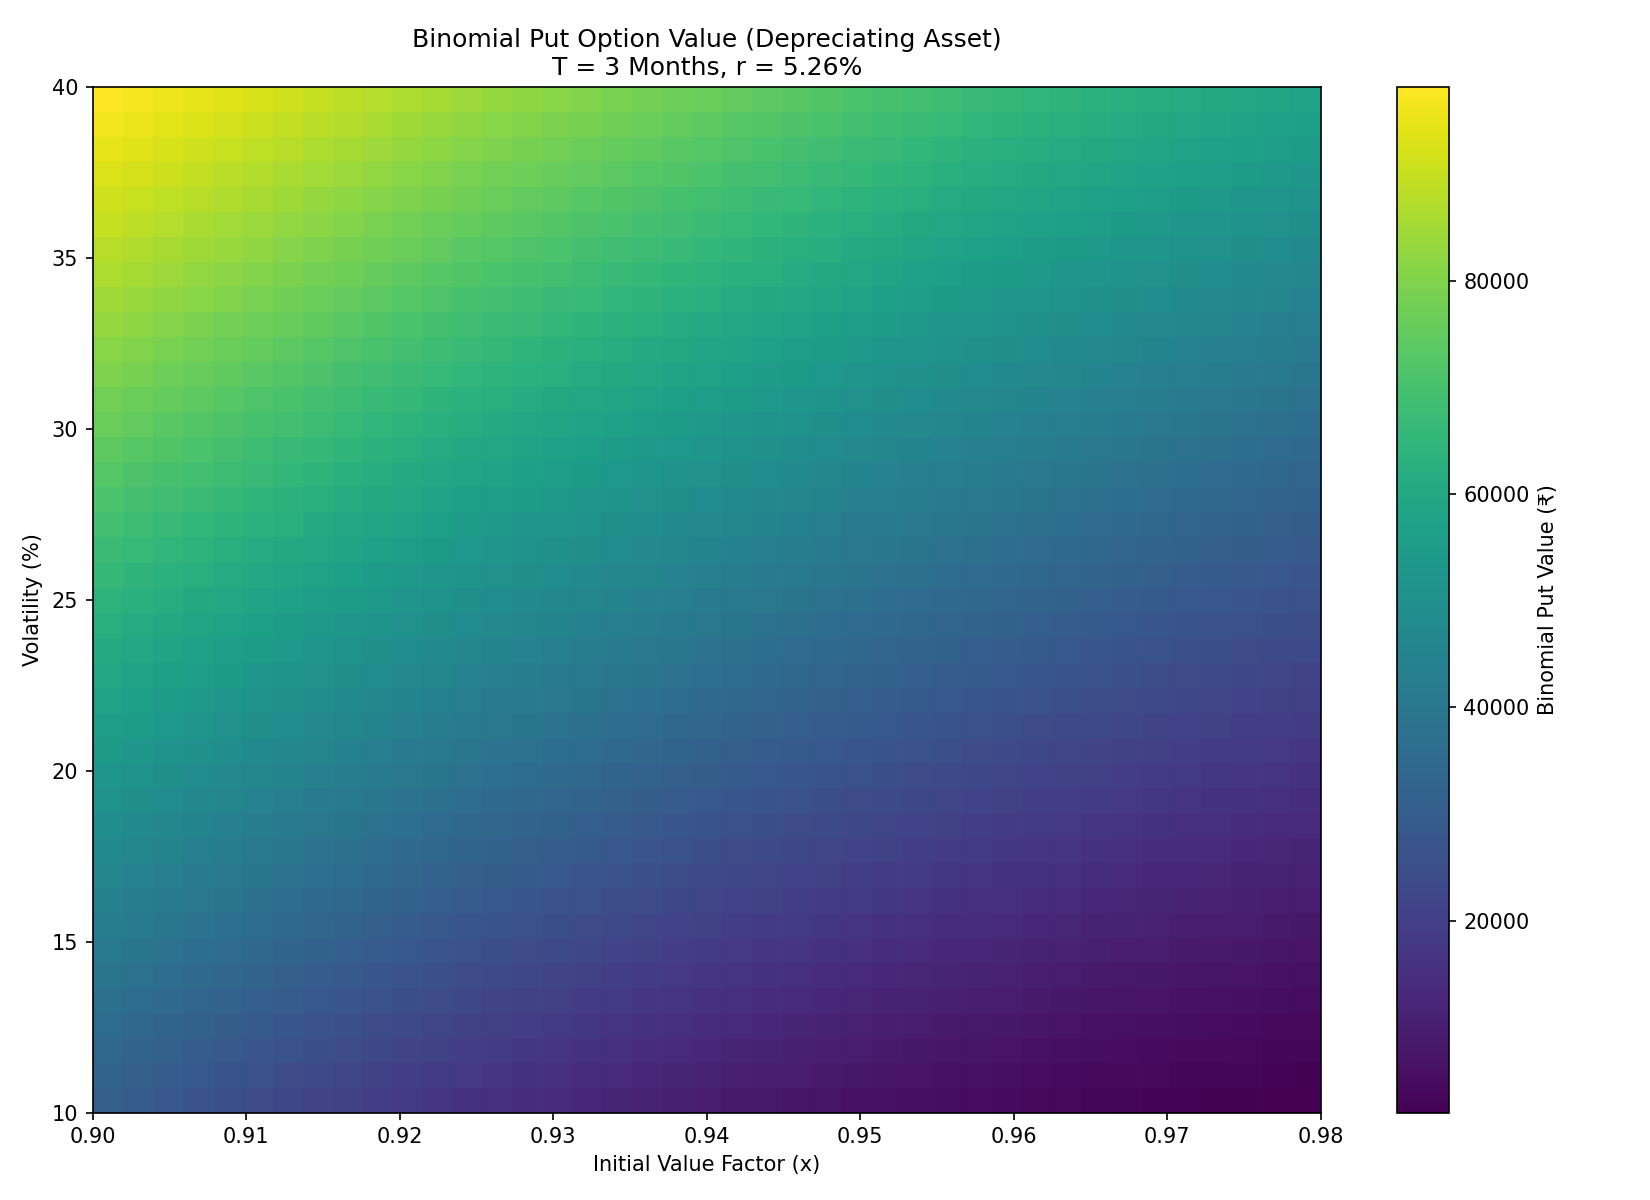
\includegraphics[width=0.85\textwidth]{fig_cell2.png}
    \caption{Binomial put option value across initial value factor ($x$) and volatility ($\sigma$), with 10\% annual depreciation. $S_0 = \text{Rs.}~12{,}83{,}903$, $K = \text{Rs.}~11{,}55{,}641$, $T = 3$ months.}
    \label{fig:binomial_heatmap}
\end{figure}

Key observations from the heatmap:
\begin{itemize}
    \item The option value ranges from Rs.~1,988 (at $x = 0.98$, $\sigma = 10\%$) to Rs.~98,159 (at $x = 0.90$, $\sigma = 40\%$).
    \item Higher volatility and lower initial value both increase the option value, consistent with standard put option theory.
    \item At low $x$ values, where the car's initial value is closer to the buyback price, the option is near or at the money and derives most of its value from volatility.
\end{itemize}


\subsubsection{Binomial Tree Visualisation}

Figure~\ref{fig:binomial_tree} shows the full binomial tree for the base case ($\sigma = 0.30$, $N = 100$). Nodes where the put is in the money ($K > S$) are highlighted with stronger opacity, while out-of-the-money nodes appear faded. The dashed line marks the strike/buyback price.

\begin{figure}[H]
    \centering
    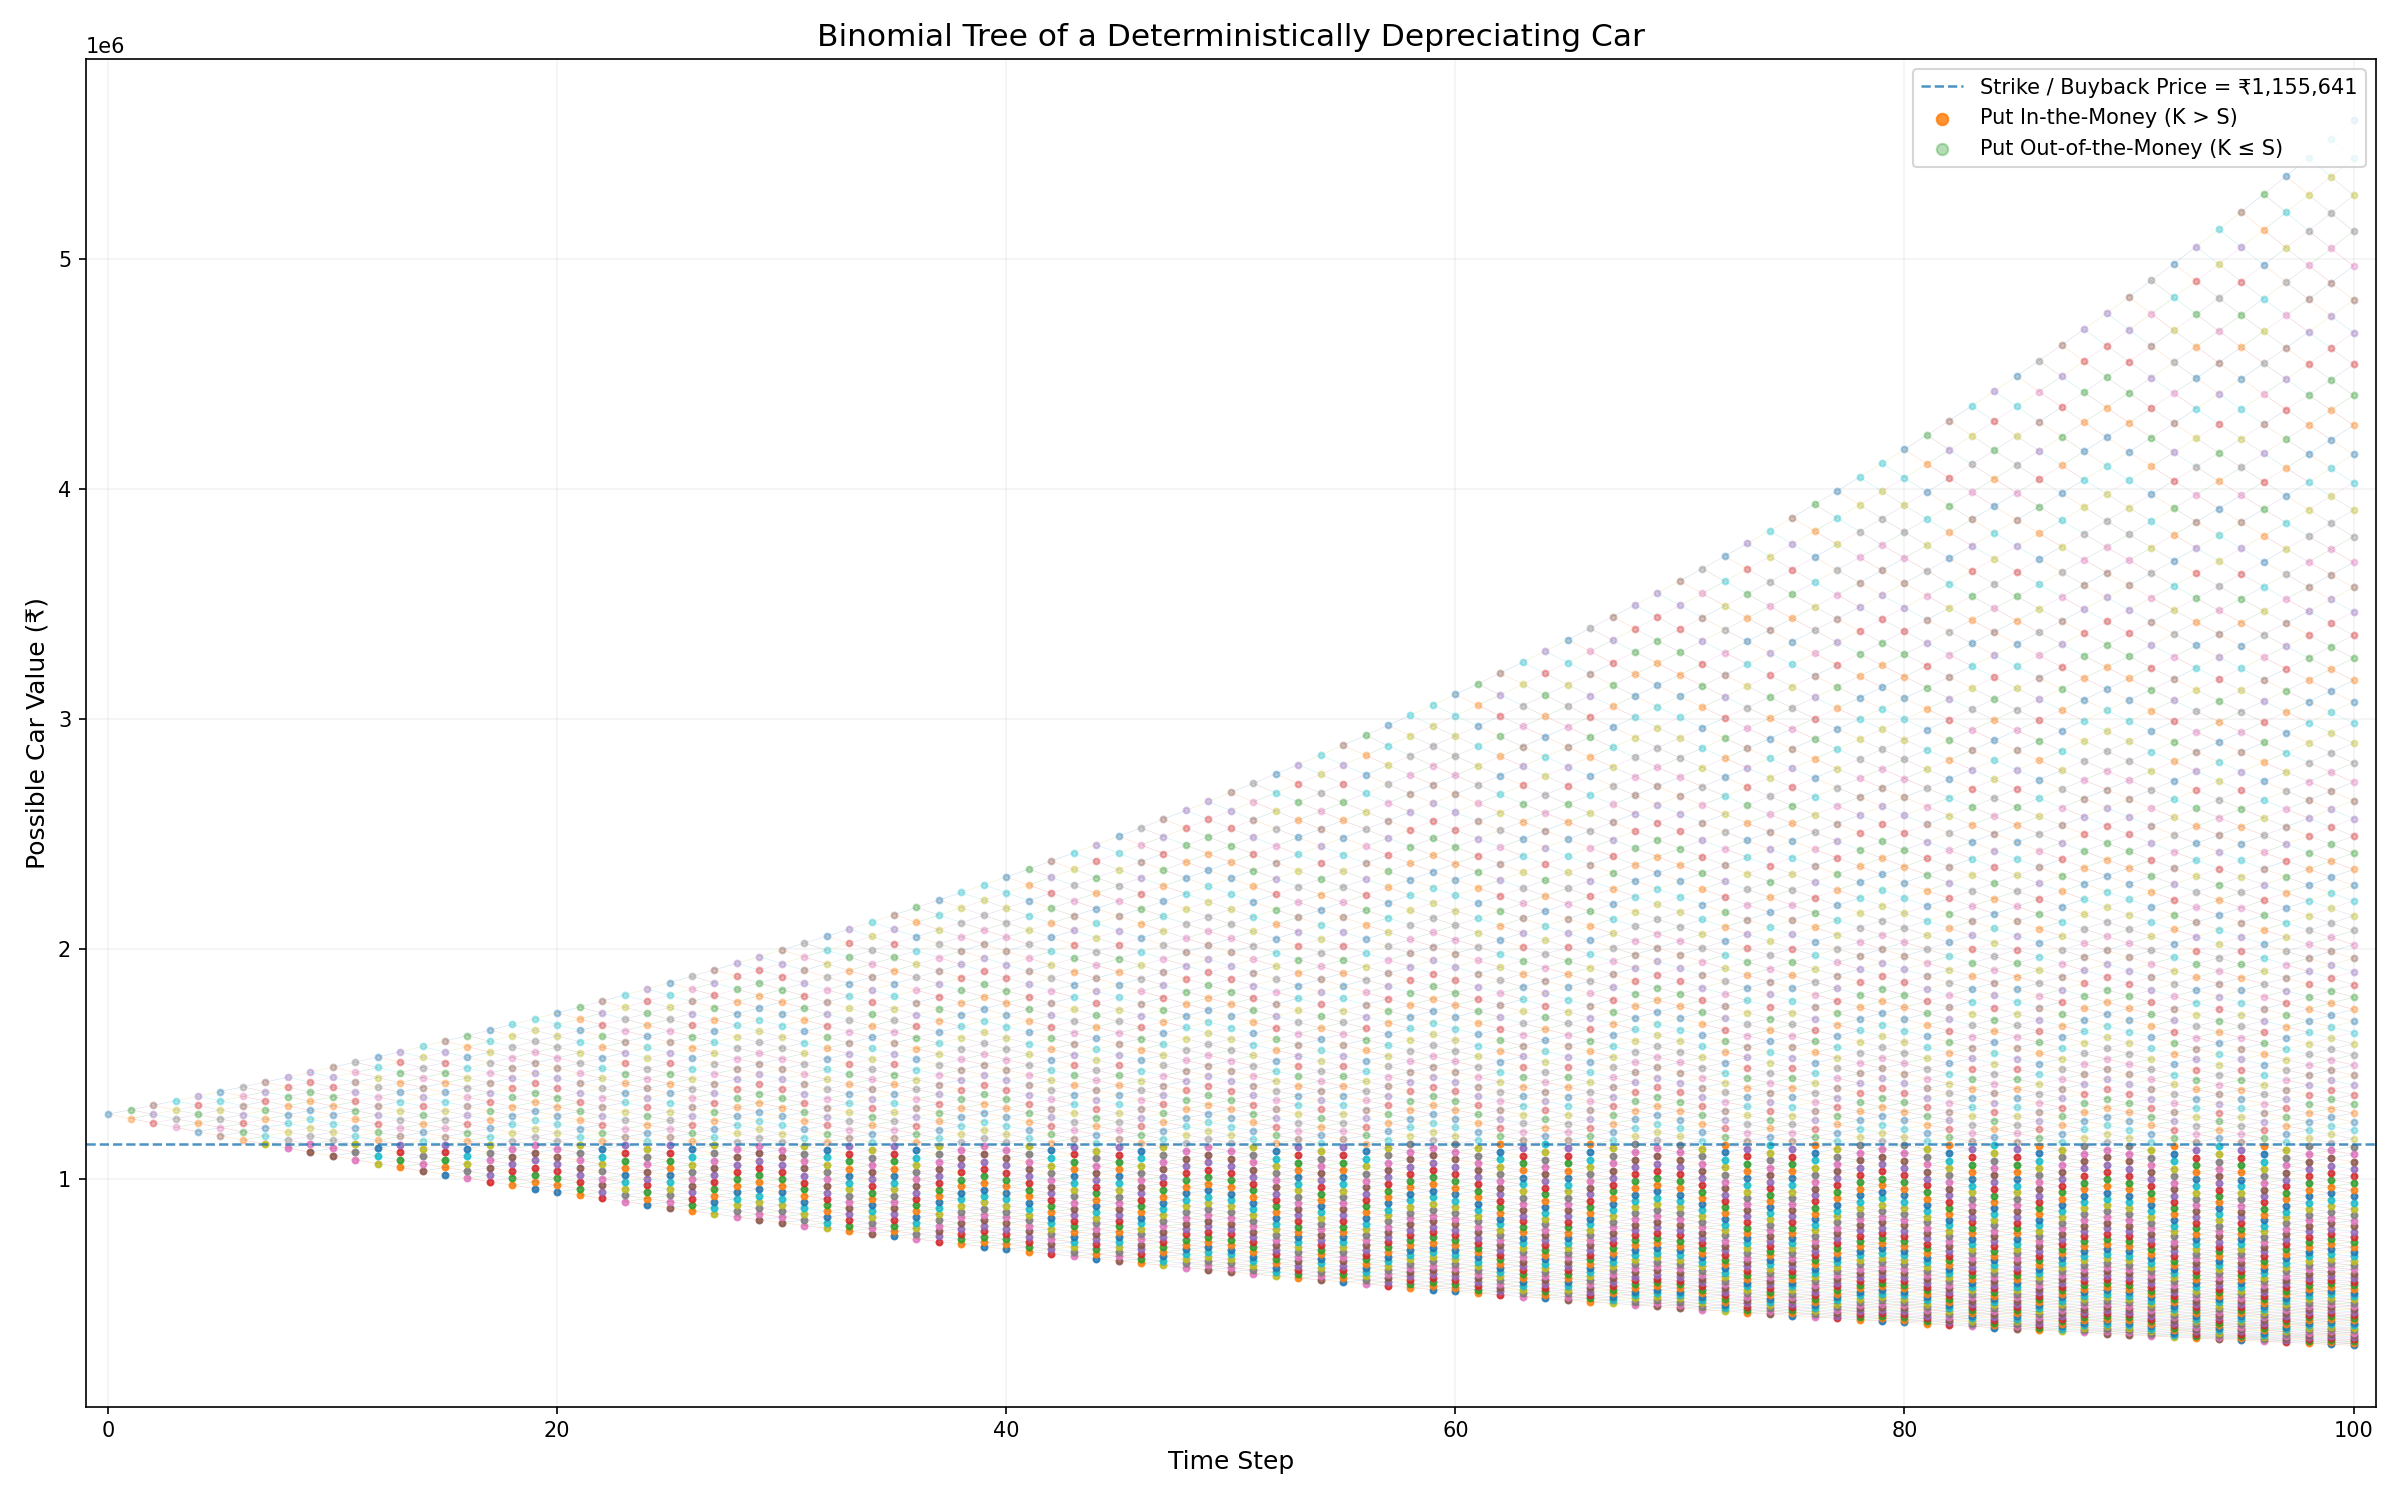
\includegraphics[width=0.95\textwidth]{fig_cell3.png}
    \caption{Binomial tree of a deterministically depreciating car. The downward drift due to depreciation is clearly visible. The tree is asymmetric in rupee terms because percentage changes are symmetric but rupee changes are not: the lattice fans out more on the upside while the downside is bounded by zero.}
    \label{fig:binomial_tree}
\end{figure}

The tree visualisation communicates two things simultaneously: the \emph{uncertainty} (fan-out of possible prices) and the \emph{depreciation} (gradual downward drift of the central tendency). The strike price line at Rs.~11,55,641 clearly delineates the region where the buyback guarantee would be exercised.


% ------------------------------------------------------------
\subsection{Pricing by Black-Scholes-Merton Formula (Standard)}
\label{sec:pricing_bsm_std}
% ------------------------------------------------------------

We now apply the Black-Scholes-Merton (BSM) closed-form solution for a European put option \cite{blackscholes1973, merton1973}.

\subsubsection{The BSM Put Formula}

The Black-Scholes price of a European put is:
\begin{equation}
    P = K \, e^{-rT} \, N(-d_2) \;-\; S_0 \, N(-d_1)
\end{equation}
where:
\begin{align}
    d_1 &= \frac{\ln(S_0/K) + (r + \tfrac{1}{2}\sigma^2)\,T}{\sigma\sqrt{T}} \\[6pt]
    d_2 &= d_1 - \sigma\sqrt{T}
\end{align}
and $N(\cdot)$ is the cumulative standard normal distribution function.

\subsubsection{BSM Heatmap (No Depreciation)}

Figure~\ref{fig:bsm_heatmap} shows the BSM put value across a grid of initial car values and volatilities, without accounting for depreciation.

\begin{figure}[H]
    \centering
    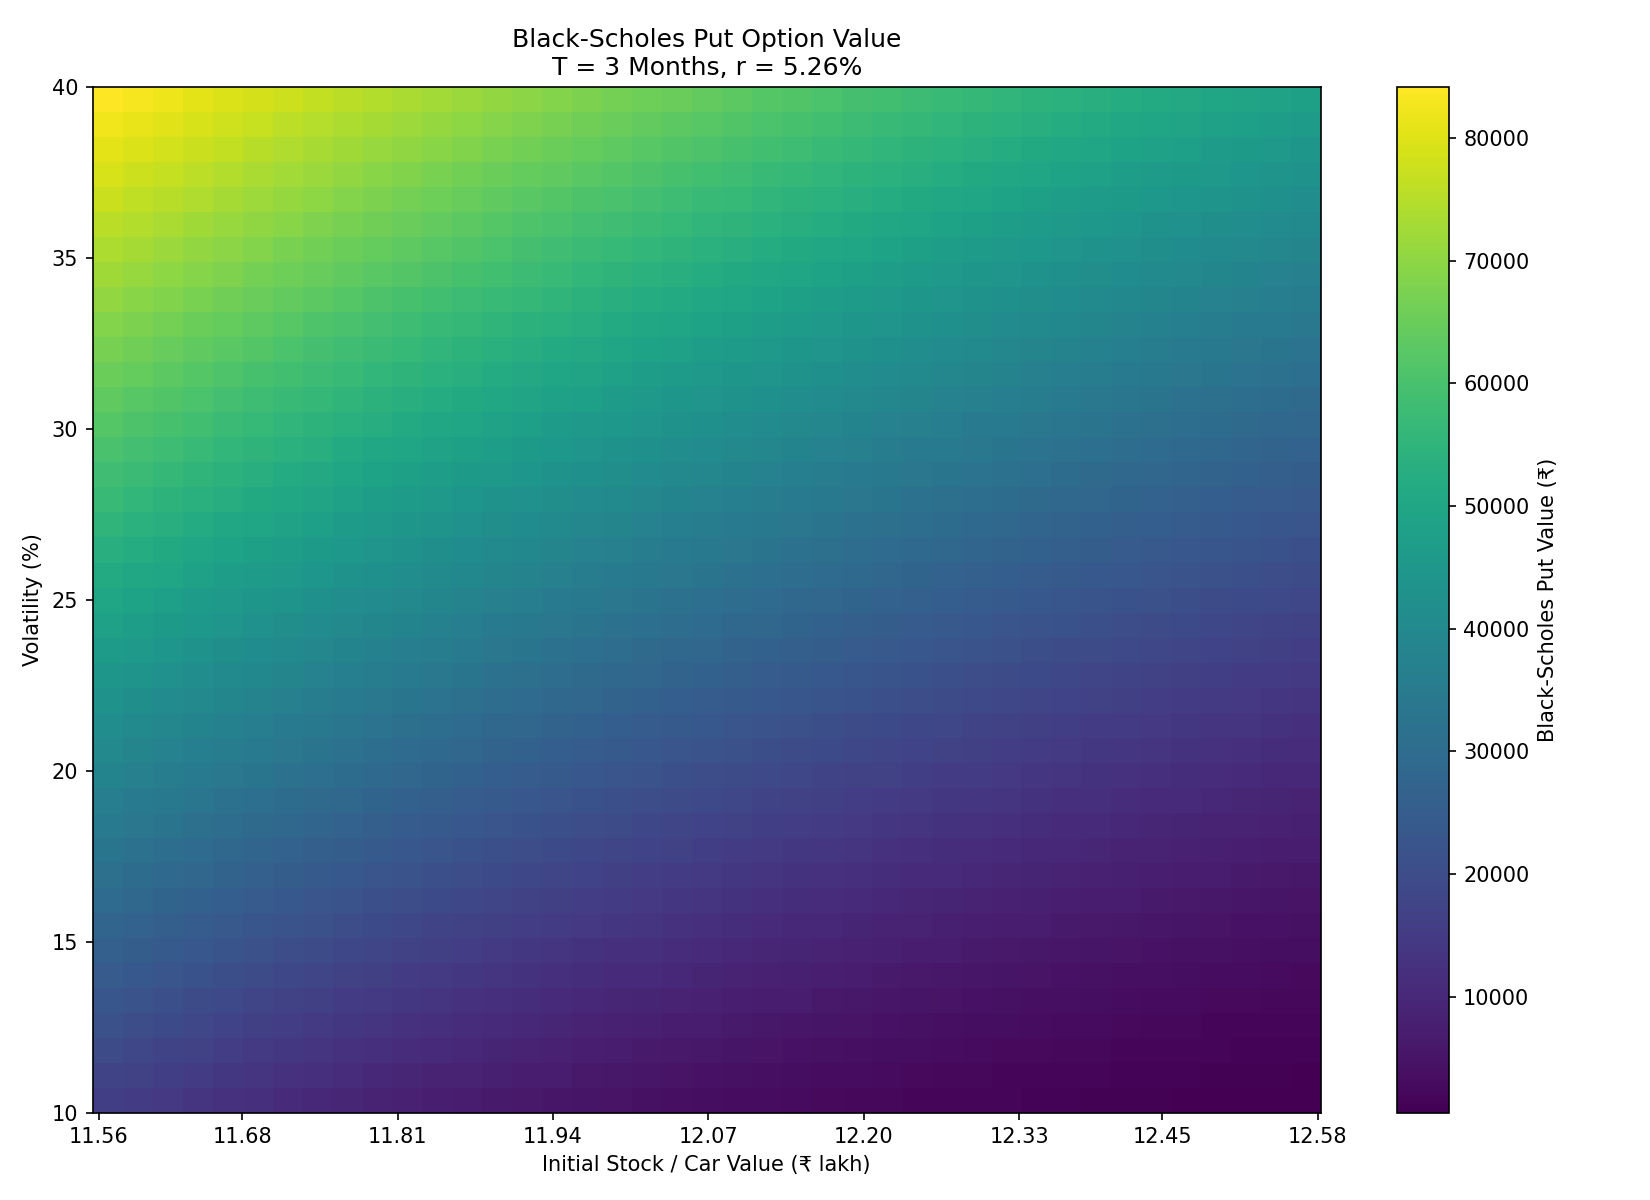
\includegraphics[width=0.85\textwidth]{fig_cell4.png}
    \caption{Black-Scholes put option value across initial car value and volatility. $T = 3$ months, $K = \text{Rs.}~11{,}55{,}641$, $r = 5.26\%$. No depreciation.}
    \label{fig:bsm_heatmap}
\end{figure}

Sample BSM put values at $\sigma = 25\%$:
\begin{itemize}
    \item At $S = \text{Rs.}~12{,}83{,}903$: Put value $\approx$ Rs.~13,905
    \item At $S = \text{Rs.}~12{,}19{,}708$ (i.e.\ $x = 0.95$): Put value $\approx$ Rs.~27,493
    \item At $S = \text{Rs.}~11{,}55{,}641$ (at-the-money): Put value $\approx$ Rs.~49,983
\end{itemize}

The overall heatmap range spans from Rs.~560 to Rs.~84,156.


% ------------------------------------------------------------
\subsection{Pricing by Black-Scholes-Merton with Depreciation}
\label{sec:pricing_bsm_dep}
% ------------------------------------------------------------

Just as we modified the binomial model, we can incorporate deterministic depreciation into the BSM framework. The key insight is to treat depreciation as a \emph{continuous proportional decay rate}, analogous mathematically to a continuous dividend yield.

\subsubsection{Converting Depreciation to a Continuous Rate}

Our binomial model assumes $S_t = S_0 (1 - 0.10)^t = S_0 (0.9)^t$. We can express this equivalently as:
\[
S_t = S_0 \, e^{-qt}
\]
where:
\begin{equation}
    q = -\ln(1 - \delta) = -\ln(0.9) \approx 0.10536 = 10.536\% \text{ p.a.}
\end{equation}

This is slightly higher than 10\% because we are converting an annual multiplicative 10\% decline into a continuously compounded rate.

\subsubsection{Modified BSM Put Formula}

The depreciation-adjusted BSM put formula becomes:
\begin{equation}
    P = K \, e^{-rT} \, N(-d_2) \;-\; S_0 \, e^{-qT} \, N(-d_1)
\end{equation}
where:
\begin{align}
    d_1 &= \frac{\ln(S_0/K) + (r - q + \tfrac{1}{2}\sigma^2)\,T}{\sigma\sqrt{T}} \\[6pt]
    d_2 &= d_1 - \sigma\sqrt{T}
\end{align}

This is mathematically equivalent to pricing a put on a dividend-paying stock, where the continuous depreciation rate $q$ plays the role of the continuous dividend yield \cite{merton1973}. The drift of the underlying under the risk-neutral measure becomes $(r - q)$ rather than $r$.

\subsubsection{BSM with Depreciation: Heatmap}

Figure~\ref{fig:bsm_dep_heatmap} shows the BSM put value with 10\% annual depreciation built in.

\begin{figure}[H]
    \centering
    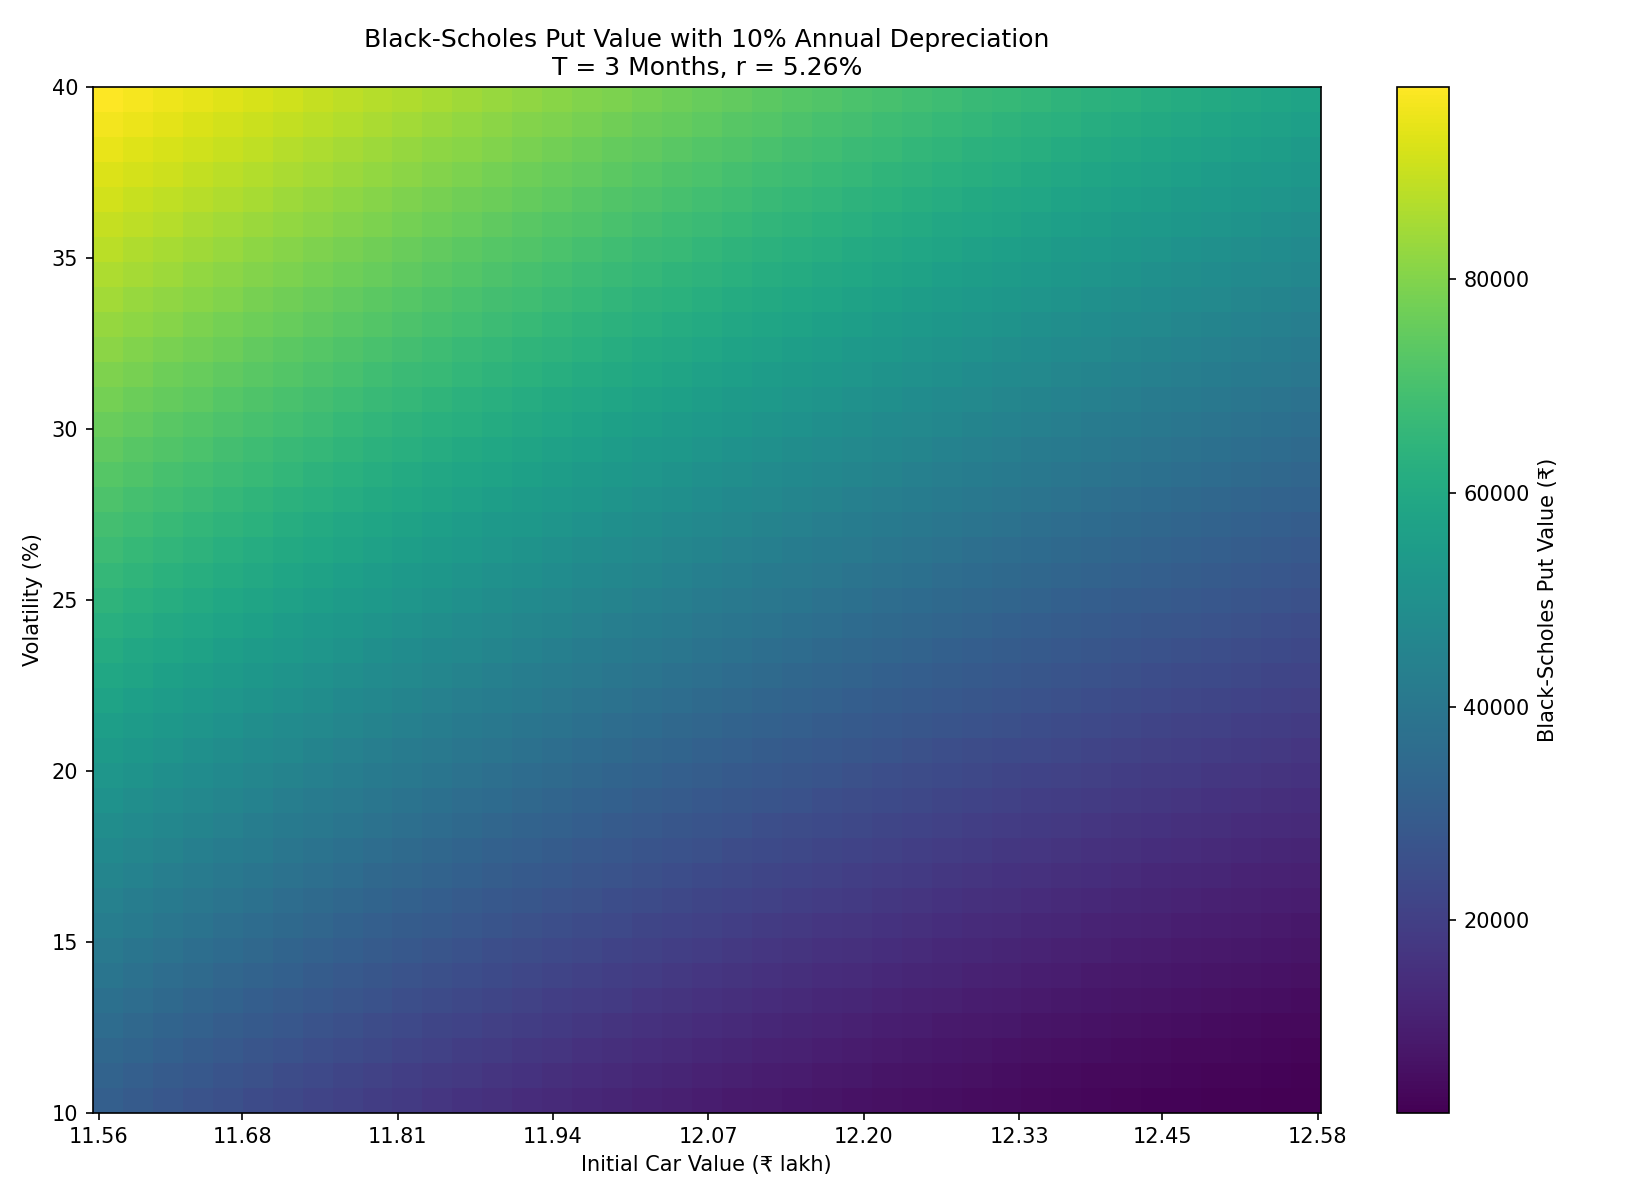
\includegraphics[width=0.85\textwidth]{fig_cell5.png}
    \caption{Black-Scholes put value with 10\% annual depreciation. $T = 3$ months, $K = \text{Rs.}~11{,}55{,}641$, $r = 5.26\%$. Depreciation enters as a continuous decay rate $q = 10.536\%$.}
    \label{fig:bsm_dep_heatmap}
\end{figure}

Sample BSM put values with depreciation at $S_0 = \text{Rs.}~12{,}83{,}903$:

\begin{table}[H]
\centering
\caption{BSM put values with 10\% depreciation at $S_0 = \text{Rs.}~12{,}83{,}903$}
\begin{tabular}{@{}cc@{}}
\toprule
\textbf{Volatility} & \textbf{Put Value (Rs.)} \\
\midrule
10\% & 768 \\
20\% & 11,539 \\
25\% & 20,020 \\
30\% & 29,502 \\
40\% & 50,112 \\
\bottomrule
\end{tabular}
\end{table}

The heatmap shows option values ranging from Rs.~1,996 to Rs.~97,984, closely matching the binomial model results and confirming convergence between the two pricing approaches. This provides a useful validation: when both models incorporate the same economic assumptions, deterministic depreciation and the same volatility, they produce nearly identical option values.


\newpage
% ------------------------------------------------------------
\subsection{Buyback Option as a Right to Abandon}
\label{sec:abandon}
% ------------------------------------------------------------

The buyback guarantee can also be framed as a \emph{right to abandon}. In real-options theory, the right to abandon an investment is valued as a put option on the project's value with the salvage/exit value as the strike price \cite{dixitpindyck1994, myers1977}.

For a Spinny customer, buying a used car is an ``investment'' in a depreciating asset. The buyback guarantee provides a guaranteed exit route: if the car's market value drops below the buyback price, or if the customer simply wants out, they can exercise their ``abandonment option'' and recover the guaranteed amount. This is analogous to how a firm might abandon a failing project and recover the liquidation value of its assets.

The total value of the car plus the embedded buyback guarantee is:
\begin{equation}
    \text{Total Security Value} = S_0 + P_0
\end{equation}
and therefore:
\begin{equation}
    \text{Value of Embedded Put} = \text{Total Security Value} - S_0
\end{equation}

For our base case with the standard binomial model, this gives a total security value of Rs.~13,06,214, meaning the buyback guarantee adds approximately Rs.~22,311 of value to the purchase (at $\sigma = 30\%$).


% ------------------------------------------------------------
\subsection{Consolidating the Pricing}
\label{sec:consolidation}
% ------------------------------------------------------------

Table~\ref{tab:consolidation} summarises the put option values obtained from the different pricing approaches for the Mahindra Bolero Neo Plus P10 ($S_0 = \text{Rs.}~12{,}83{,}903$, $K = \text{Rs.}~11{,}55{,}641$, $r = 5.26\%$, $T = 3$ months).

\begin{table}[H]
\centering
\caption{Consolidated option values across pricing methods}
\label{tab:consolidation}
\begin{tabular}{@{}lcc@{}}
\toprule
\textbf{Method} & \textbf{Volatility} & \textbf{Put Value (Rs.)} \\
\midrule
Fundamental (discounted depreciation baseline) & -- & 32,941 \\
Standard Binomial ($N = 100$) & 30\% & 22,311 \\
BSM (no depreciation) & 25\% & 13,905 \\
BSM (with depreciation) & 25\% & 20,020 \\
BSM (with depreciation) & 30\% & 29,502 \\
BSM (with depreciation) & 15\% & 4,746 \\
\bottomrule
\end{tabular}
\end{table}

At the base-case volatility of 15\% (from the listing parameters), the BSM model with depreciation gives a value of approximately Rs.~4,746, modest but not negligible, and well below the Rs.~32,941 fundamental baseline from Section~\ref{sec:pricing_fundamental}. This is a useful sanity check in itself: because the fundamental baseline ignores volatility altogether, it need not sit below the stochastic estimates at every volatility level, and the crossover shows how much of the option's value at low volatility is coming from the deterministic depreciation drift rather than from uncertainty. At higher volatilities (25--30\%), which may better reflect the true uncertainty in used-car resale values, the option value rises to Rs.~20,000--29,500, comparable to, and at 30\% slightly below, the fundamental baseline.

Both the binomial and BSM models confirm that the buyback guarantee carries material value when volatility is moderate to high, and that incorporating depreciation significantly increases the put value relative to a standard model.

It is also useful to relate these model values back to what the option actually costs the customer. Section~\ref{sec:buyback_offer} noted that Spinny charges a flat Rs.~5,000 fee for the buyback assurance, regardless of the vehicle. At the base-case volatility of 15\%, our depreciation-adjusted BSM value of roughly Rs.~4,746 is close to this fee, which suggests that at low volatility the flat charge approximately covers the financial option value. At volatilities of 25--30\%, more representative of the swings actually observed in the used-car market, the fair value of the put rises to Rs.~20,000--29,500, several times the flat fee. This points to Spinny's buyback fee being priced conservatively, or even as a loss leader, for vehicles or market conditions where resale values are genuinely volatile, while remaining roughly break-even in calmer conditions.

From Spinny's perspective, this option is a cost embedded in every sale. Spinny would price it factoring in:
\begin{itemize}
    \item The expected depreciation and buy-sell spread.
    \item Inspection and reconditioning costs upon return.
    \item The probability that a customer actually exercises the buyback (exercise rate).
    \item The cost of capital tied up in the guaranteed repurchase commitment.
\end{itemize}

The fact that Spinny sets the buyback price at roughly 90\% of the selling price (a 10\% haircut) is consistent with covering the expected depreciation over the guarantee window plus a margin for operational costs and adverse selection.


% ============================================================
\section{Conclusion}
\label{sec:conclusion}
% ============================================================

This report demonstrates that Spinny's buyback guarantee is economically equivalent to a European put option on a deterministically depreciating asset. Applying three pricing methods, fundamental analysis, the binomial tree model (with deterministic depreciation), and the Black-Scholes-Merton formula (both standard and depreciation-adjusted), we showed that the guarantee carries non-trivial value, particularly when the used-car market's volatility is moderate to high.

The key insight from incorporating deterministic depreciation is that it significantly increases the put option value relative to a standard model that ignores depreciation. This makes sense intuitively: a depreciating asset is more likely to fall below the guaranteed floor, making the put more valuable to the holder. In our modified model, the car's value at each point in time is decomposed as:
\[
S_t = S_0 \cdot (1 - \delta)^t \cdot u^j \cdot d^{(i-j)}
\]
where the first factor captures the deterministic decline and the second captures stochastic market movements.

For the Mahindra Bolero Neo Plus P10 (2024) listed at Rs.~12,83,903 with a buyback guarantee of Rs.~11,55,641, our models yield option values ranging from a few hundred rupees (at low volatilities) to over Rs.~98,000 (at high volatilities and low initial values). At realistic volatilities of 15--25\%, the option value sits in the range of Rs.~4,700--20,000.

For Spinny, the buyback guarantee serves a dual purpose. It is both a marketing tool, reducing buyer anxiety and increasing conversion rates, and a financial obligation that must be carefully priced. Our analysis provides a framework for understanding the cost of this obligation and how it varies with the key parameters of asset value, volatility, and time.


% ============================================================
\section{Acknowledgements}
% ============================================================

We thank the course instructor, Prof. Thillai A Rajan and the TA, Ajith for their guidance and help in the project. We also thank the employees of Spinny for engaging with us and eventually giving us some useful information.


% ============================================================
\section{Code, Data, and Other Resources}
% ============================================================

All code used for the option pricing models and visualisations is available on Github. The repository contains:

\begin{itemize}
    \item Standard binomial put option pricing model.
    \item Binomial model with deterministic asset depreciation.
    \item Heatmap sensitivity analysis (binomial).
    \item Binomial tree visualisation.
    \item Black-Scholes-Merton put pricing (standard and with depreciation).
    \item BSM heatmap sensitivity analysis.
\end{itemize}

The code is written in Python using \texttt{numpy}, \texttt{scipy}, and \texttt{matplotlib}, and can be found at \url{https://github.com/paradoxically-loki/sem9/tree/main/ms5612}.


% ============================================================
% BIBLIOGRAPHY
% ============================================================
\newpage
\begin{thebibliography}{99}

\bibitem{blackscholes1973}
Black, F. and Scholes, M. (1973).
\textit{The Pricing of Options and Corporate Liabilities}.
\textit{Journal of Political Economy}, 81(3), 637--654.

\bibitem{merton1973}
Merton, R.C. (1973).
\textit{Theory of Rational Option Pricing}.
\textit{The Bell Journal of Economics and Management Science}, 4(1), 141--183.

\bibitem{crr1979}
Cox, J.C., Ross, S.A. and Rubinstein, M. (1979).
\textit{Option Pricing: A Simplified Approach}.
\textit{Journal of Financial Economics}, 7(3), 229--263.

\bibitem{dixitpindyck1994}
Dixit, A.K. and Pindyck, R.S. (1994).
\textit{Investment under Uncertainty}.
Princeton University Press.

\bibitem{hull2022}
Hull, J.C. (2022).
\textit{Options, Futures, and Other Derivatives} (11th ed.).
Pearson.

\bibitem{myers1977}
Myers, S.C. (1977).
\textit{Determinants of Corporate Borrowing}.
\textit{Journal of Financial Economics}, 5(2), 147--175.

\bibitem{entrackr2025}
Entrackr (2025).
\textit{Spinny posts Rs 4,657 Cr revenue in FY25; cuts losses by 28\%}.
Retrieved from \url{https://entrackr.com/fintrackr/spinny-posts-rs-4657-cr-revenue-in-fy25-cuts-losses-by-28-10509574}.

\bibitem{tracxn2026}
Tracxn (2026).
\textit{Spinny -- Company Profile, Funding, Competitors \& Financials}.
Retrieved from \url{https://tracxn.com/d/companies/spinny/}.

\bibitem{forbesindia2023}
Forbes India (2023).
\textit{How Spinny emerged as a dark horse in the race to win the used car market}.
% Retrieved from \url{https://www.forbesindia.com/article/take-one-big-story-of-the-day/rearview-mirror-lost-alignment-and-a-leap-of-faith-how-spinny-emerged-as-a-dark-horse/85135/1}.

\bibitem{spinnyassured}
Spinny (2026).
\textit{Spinny Assured -- The sure road to Car Joy}.
Retrieved from \url{https://www.spinny.com/spinny-assured/}.

\bibitem{spinnybuyback}
Spinny (2026).
\textit{What is Spinny BuyBack?}
Retrieved from \url{https://support.spinny.com/hc/en-gb/articles/360052602031-What-is-Spinny-BuyBack}.

\bibitem{spinnybuybackblog}
Spinny (2021).
\textit{Spinny Used Car Buyback Programme: Commit Less, Drive More}.
Retrieved from \url{https://www.spinny.com/blog/spinny-buyback/}.

\end{thebibliography}

\end{document}